\section{PACT}\label{sec:PACT}
When designing an interactive system it is important to be human-centered, since it is the users who at the end determines the use of a given system through their interactions with it.
\\\indent
Depending on how well designers have implemented a way to convey their conception of a given system, different users will interpret it differently. 
Their interpretation being based on individual understanding and knowledge, regulates the users interactions with the system and thereby determines what it actually does see \cref{fig:PACT-SystemImage}.

\begin{figure}[H]
	\centering
	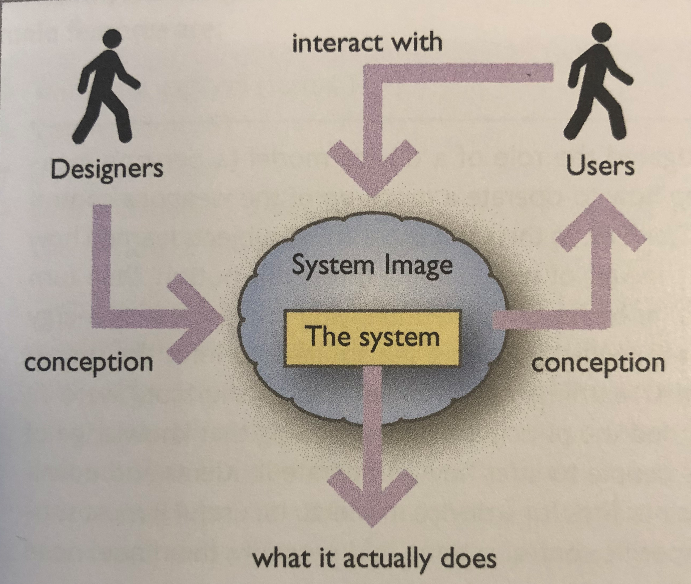
\includegraphics[width=0.5\textwidth]{billeder/SystemImage-Benyon.png}
	\caption{\textit{The System Image from {\color{red}Benyon side 31}}}
	\label{fig:PACT-SystemImage}
\end{figure}


To help understanding and analyzing the people and their relation to the problem, the PACT framework is used.
PACT is an acronym for ''{\itshape{people}}'', ''{\itshape{activities}}'', ''{\itshape{contexts}}'' and ''{\itshape{technologies}}''.
These four elements in the framework will be explained further in the subsection \ref{sec:PACT-framework} below.

\subsection{The PACT framework}\label{sec:PACT-framework}
\subsubsection*{People}

\subsubsection*{Activities}

\subsubsection*{Contexts}

\subsubsection*{Technologies}


\subsection{PACT analysis}\label{sec:PACT-analysis}
Based on the interview
\todo{maybe interviews depending on whether or not we change it after further interviews}
with Pia,
% conslutant and acting quality chief at JBJ,
{\color{red} section XX}, the PACT analysis for the project described in this report is as follows.

\subsubsection*{People}

There are four main groups of people; the quality manager, the secretary, department heads and everyday workers.
This is a heterogeneous group with different levels of IT experience ranging from no skills with IT and therefore cautious about it, to the level of everyday office work.
The group also has different levels of domain expertise ranging from no to expert which needs to be considered. The quality manager is a domain expert and therefore has different needs of the system than the everyday worker with no expertise.
\newline
Furthermore, issues such as colorblindness, other eye handicap as well as bad memory need to be considered when designing the system and interface.


\subsubsection*{Activities}
The overall activities is to manage, update and access a handbook mostly the newest version but also possibly older versions as well. It is needed to uphold the standards from the government to retain the companies certifications.
This is a well defined activity
which takes place at least yearly, though sometimes more often.
%In the case of JBJ it happens more often
When doing the activities users may experience interruptions and should therefore be simple to use and easy to get back to.
Additionally, the activities is mostly done alone but may be done in collaboration with others, though this is not required.
\newline
The data to be entered into the system are mostly larger data entries and possibly many of such.
the system is not safety critical but integrity is an important aspect.

\subsubsection*{Contexts}


\subsubsection*{Technologies}














